\section{Antennentheorie}
Eine hypothetische verlustlose Antenne, die gleichmässig in alle Raumrichtungen abstrahlt beziehungsweise aus allen Richtungen empfängt, wird isotroper Strahler oder Kugelstrahler genannt. Als Sendeantenne erzeugt sie eine Kugelwelle mit sphärischen Phasenfronten. Im Abstand gilt winkelunabhängig folgende Leistungsdicht:
%\[S=\frac{P_{S}}{4r\]
\[S=\frac{P_{S}}{4 \pi r^{2}}\]
wobei $P_{S}$ die gasamt abgestrahlte Wirkleistung bezeichnet.

\subsection{elementarer Antennen Dipole}
\subsubsection{Hertzscher Dipol}
Ein elektrisch kurzer Linearstrahler der länge $l<<\frac{\lambda_{0}}{4}$ kann als konzentriertes Bauelement betrachte werden. Auf seiner gesamten Länge kann die komplexe Amplitude $\underline{I}$ eine räumlich konstante Stromverteilung, die zeitlich sinusförmig schwingt, annehen.
\subsubsection{Fitzgeraldscher Dipol}
\subsection{Nahfeld und Fernfeld}

Im Fernfeld steht das E und H Feld senkrecht  im 90$^\circ$Winkel aufeinander. Die Wellenfront der beiden Felder bewegt sich in Ausbreitungsrichtung wie eine senkrechte Ebene.\\
Die minimale Distanz ab der die Annahme des Fernfeld getroffen werden kann
 lautet wir folgt:
\[do=\dfrac{2D^2}{\lambda}\]
Mit:\\d0: Minimale Distanz für die Annahme des Fernfeld Kriterium\\
D: Grösstes Antennmass in Meter\\
$\lambda$: Wellenlänge
\todo{quelle vom bild einfügen}
%https://de.wikipedia.org/wiki/Nahfeld_und_Fernfeld_%28Antennen%29
\begin{figure}[htbp]
	\centering
		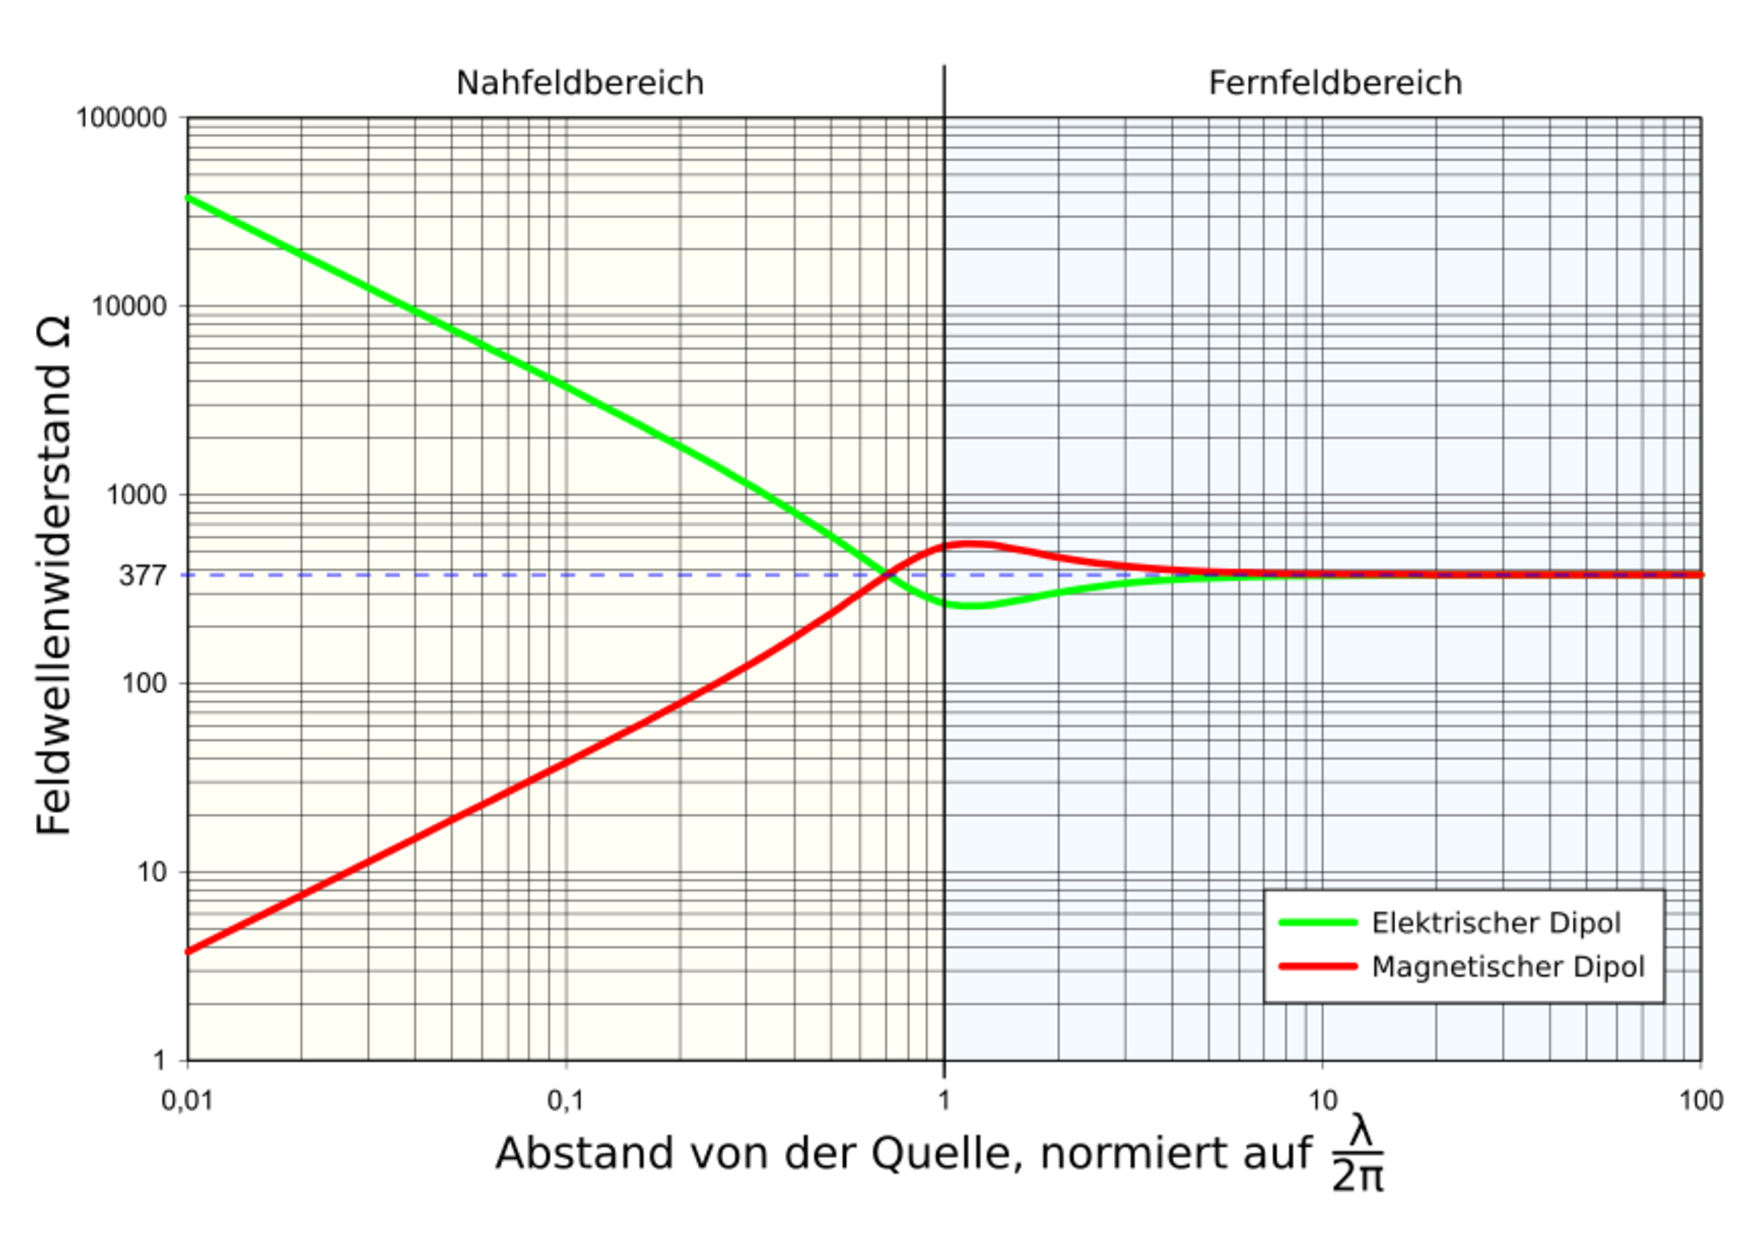
\includegraphics[width=6cm]{content/bilder/Feldwellenwiderstandsverlauf_im_Nahfeld-Fernfeld.pdf}
	\caption{Nah-Fernfeld}%
	\label{Nah-Fernfeld}
\end{figure}
\subsection{Antennenbauformen}
\subsection{symmetrisch gespiesene Antennen}


Es gibt zwei Grundantennenformen, den Hertzschen Dipol und den Fitzgeradscher Dipol. Beide sind symmetrisch gespiesene Antennen. Im Nahfeld des Hertschen Dipols überwiegt das E Feld also der kapazitive Anteil, während im Nahfeld des Fitzgeradschen Dipols das H Feld also der induktive Anteil überwiegt. Im Fernfeld sind bei beiden Antennen das H und E Feld gleich stark und nehmen mit zunehmendem Abstand $1/r$ab. \\
Die Ausrichtung des E und H Feld sind bei den beiden Antennen verschieden. \\
Das E Feld eines Hertschen Dipols ist im Fernfeld gleich polarisiert wie der Dipol. \\
Genau umgekehrt ist das Feld des Fitzgeralschen Dipols. Das H Feld ist in der selben Ebene wie der Dipol. 

\begin{itemize}
\item Bauform
\item el. mag Feld Ausrichtung
\item Impedanz der $\lambda /2 $ Antenne
\item Beschreibung des Feld
\item el. mag Feld Ausrichtung
\item Impedanz der $\lambda /2 $ Antenne
\item Richtcharakteristik
\end{itemize}
\subsubsection{$\lambda /2 $ Dipol Antenne}
Die $\lambda /2 $ Dipol Antenne ist eine der am Meisten eingesetzten Antennen. In diesem Abschnitt wird die Dipolantenne mit einer sehr dünnen Radius  deren Länge einer halben Wellenlänge entspricht betrachtet. 

Eine Dipol Antenne mit der Länge L entlang der Z-Achse orientiert ist und z = 0 ist, fliesst der Strom in der z-Richtung mit einer Amplitude, die der folgende Funktion entspricht:
$I(z)=\begin{cases}I_{0}sin[k(\frac{L}{2}-z)],& 0\le z \le \dfrac{L}{2} \\ I_{0}sin[k(\frac{L}{2}+z)], & -\dfrac{L}{2} \le z \le 0 \end{cases}$

%\begin{tikzpicture}[xscale=0.04,yscale=0.08,domain=0.125:220,samples=400]
%    \draw[->] (-10,0) -- (225,0) node[below] {$x$};
%    \draw[->] (0,-5) -- (0,45) node[left] {$y$};
%    \foreach \i in {50,100,...,200} {
%        \draw (\i,1) -- (\i,-1) node[below] {$\i$};
%    }
%    \foreach \i in {10,20,...,40} {
%        \draw (1,\i) -- (-1,\i) node[left] {$\i$};
%    }
%    \draw[blue] plot (\x,{40-0.2*\x});
%    \draw[red] plot (\x,{5/\x});
%\end{tikzpicture}

Bei einem Dipol mit der Länge  $L= \frac{\lambda}{2}$ sich einen Strombauch über dem Einspeise Punkt ausbildet und der Strom zu den Enden gegen null geht.\\
Ein Dipol mit der Länge  $L= \lambda$ bilden sich zwei  Strombauche über die ganze Länge des Dipols aus. Beim Einspeise Punkt und den beiden Enden geht der Strom gegen null.\\
Wichtig bei der Stromverteilung ist, dass der Strom  in der Zeit sinusförmig  mit der Frequenz f oszilliert. 


%Abbildung \nodepart{•}; Stromverteilungen auf endlich langen Dipol-Antennen.

Die Eingangsimpedanz eines Dipols ist Abhängigkeit von seiner Länge. Man beachte, dass die Eingangsimpedanz wird als Z = R + jX, wobei R der Widerstand und die Reaktanz X angegeben. Die Reaktanz X ist steht für die im Nahfeld gespeicherte Feldenergie.

%Abbildung 2. Eingangsimpedanz in Abhängigkeit von der Länge (L) einer Dipolantenne.

Man beachte, dass für sehr kleine Dipolantennen, ist die Eingangsimpedanz kapazitiv ist, das heisst, die Impedanz durch eine negative Reaktanz-Wert (und eine relativ kleine reale Impedanz oder Widerstand) dominiert. Wir der Dipol länger, so erhöht sich der Eingangswiderstand, zusammen mit der Reaktanz. Bei etwas weniger als $L=\frac{\lambda}{2}$ hat die Antenne Nulldurchgang des Imaginärteils.

Wenn die Länge des Dipol-Antenne ist nahe der Wellenlänge ist, wird die Eingangsimpedanz unendlich. Als einfachere Erklärung, kann der Stromverteilung einer $L = \lambda$ langen Antenne betrachtet werden. ES ist ersichtlich, dass bei der Einspeisestelle der Strom gegen Null geht. Unter Berücksichtigung, dass der Strom nach dem Ohmschen Gesetz $I = \frac{U}{R}$ ist, so ist naheliegen, dass der Widerstand gegen unendlich gehen muss. 

Im nächsten Abschnitt werden wir das Strahlungsmuster Dipol-Antennen zu berücksichtigen.


Strahlungsdiagramme für die Dipol-Antennen

Die weit Felder aus einer Dipolantenne der Länge L sind gegeben durch:
\[E_{\theta}=\frac{j\eta I_{0} e^{-jkr}}{2\pi r}\frac{cos(\frac{kL}{2}cos(\theta))-cos(\frac{kL}{2}))}{sin(\theta)}\]

\[H_{\Phi}=\frac{E_{\Theta}}{\eta}\]

Die normierten Strahlungsmuster für Dipolantennen verschiedener Längen sind in Abbildung 3 dargestellt.


Abbildung 3. normalisierte Strahlungsmuster für die Dipol-Antennen der angegebenen Länge.

Die Full-Wellenlängen-Dipol-Antenne ist richtungs als die kürzere Viertelwellenlängen-Dipol-Antenne. Dies ist ein typisches Ergebnis der Antennentheorie: es dauert eine größere Antenne allgemein Richt erhöhen. , Die Ergebnisse sind jedoch nicht immer offensichtlich. Das 1,5-Wellenlängen-Dipol-Muster ist ebenfalls in Figur 3. Anmerkung aufgetragen dass dieses Muster ein Maximum bei etwa +45 und -45 Grad.

Die Dipolantenne ist symmetrisch, wenn azimutal angesehen (um die lange Achse des Dipols); als Ergebnis das Strahlungsmuster nicht eine Funktion des Azimutwinkels. Damit ist die Dipolantenne ein Beispiel einer Rundstrahlantenne. Ferner hat das E-Feld nur eine Vektorkomponente und damit die Felder linear polarisiert. Wenn sie in der XY-Ebene betrachtet wird (für einen Dipol entlang der z-Achse orientiert ist), wird die E-Feld in der -y-Richtung, und folglich wird die Dipolantenne ist vertikal polarisiert.

Das 3D-Motiv für das 1-Wellenlängen-Dipol-Antenne ist in 4 gezeigt Dieses Muster ist ähnlich dem Muster für die Viertel- und Halbwellen-Dipolantenne.


Abbildung 4. Normalized 3d Strahlungsmuster für die 1-Wellenlängen-Dipol-Antenne.

Die 3D-Strahlungsmuster für die 1.5-Wellenlängen-Dipol-Antenne unterscheidet sich signifikant und wird in 5 gezeigt.


Abbildung 5. Normalized 3d Strahlungsmuster für die 1,5-Wellenlängen-Dipol-Antenne.
Das (peak) Richtcharakteristik der Dipolantenne variiert, wie in Figur 6 gezeigt.


Abbildung 6. Dipole Antenna Richtwirkung als eine Funktion der Dipollänge.

Abbildung 6 zeigt, dass bis zu etwa L = 1,25 Die Richt steigt mit der Länge. , Für größere Längen die Richtwirkung hat jedoch einen Aufwärtstrend ist aber nicht mehr monoton.

Im nächsten Abschnitt werden wir am häufigsten Dipol-Antenne, die Halbwellen-Dipol-Antenne suchen.
\begin{itemize}
\item Fusspunkt Impedanz
\item Feldausbreitung im Nahfeld
\item Feldausbreitung im Fernfeld
\item Im Nahfeld relevant
\item Richtcharakteristik
\end{itemize}
\subsubsection{Loop Antenne}
Die Loop Antenne ist eine symmetrisch gespiesene Antenne. eine Loop Antenne ist einem Fitzgeralschen Dipol nach empfunden. Die Loop Antenne wird durch eine dünne Leiterschleife mit einem Radius  $r=\dfrac{bla}{bla}$  dargestellt. \\
Im Nahfeld der Loop Antenne dominiert der xx Anteil. Das E Felde ist in der Ebene der Leiterschleife. Das H Feld erscheint 90$^\circ$Winkel zum E Feld. 
\subsection{Abstrahlcharakteristik}
\subsubsection{Monopol über leitendem Ground}
In der Praxis werden Monopolantennen über Masseflächen mit endlicher Leitfähigkeit und endlicher Grösse verwendet. Dies beeinflusst die Eigenschaften der Monopolantennen, insbesondere das  Strahlungsmuster. Die Impedanz der Monopolantenne wird minimal über einem endlichen grossen Massebene verändert. Voraussetzung hierfür ist, dass die Massebene  im Durchmesser über einige  Wellenlängen der Abstrahlfrequenz besitzt. Jedoch ist die Strahlungscharakteristik der Monopolantenne stark durch eine endliche Grösse Massebene beeinflusst. Das resultierende
 Strahlungsdiagramm strahlt in einer "schrägen" Richtung, weg von
  der horizontalen Ebene. Ein Beispiel für das Strahlungsmuster für eine 
  $\dfrac{\lambda}{4}$ 
  Monopolantenne mit einem Durchmesser der Massenfläche von 3 Wellenlängen. 
  Die  $\dfrac{\lambda}{4}$  Monopolantenn ist in der positiven z Richtung ausgerichtet.

%Strahlungsmuster der Monopolantenne aufgrund der endlichen Grösse Massebene.

Das resultierende Strahlungsmuster für diese Monopolantenne ist  omnidirektionalen. Jedoch hat die Richtung der maximalen Strahlung von der xy-Ebene in einem Winkel von dieser Ebene angehoben verändert. Im Allgemeinen gilt je  grösser Grundplatte ist, desto niedriger ist diese Richtung der maximalen Strahlung. Das bedeutet wenn die Grundebene sich gegen  unendlich nähert, so liegt die maximale  Strahlung  in der xy-Ebene.
%\cite{http://www.antenna-theory.com/antennas/monopole.php}

Der Antennengewinn ist  um 3 dB besser als eine Dipol Antenne. Da die Monopolantenne ihr Feld nur über dem perfekt leitendem Untergrund aufbaut.
%\cite{Zitat01}
%\cite{UndNochEinZitat}
%\cite{Zitat02}
\cite{sti06}
\cite{sti06}